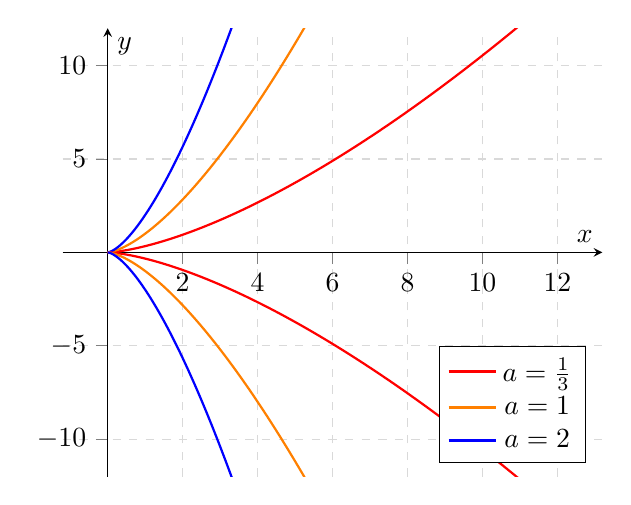
\begin{tikzpicture}
    \begin{axis}[
        legend pos=south east,
        axis x line=middle,
        axis y line=middle,
        grid = major,
        %width=9cm,
        %height=4.5cm,
        grid style={dashed, gray!30},
        xmin= 0,     % start the diagram at this x-coordinate
        xmax= 12,    % end   the diagram at this x-coordinate
        ymin=-10,     % start the diagram at this y-coordinate
        ymax= 10,   % end   the diagram at this y-coordinate
        %axis background/.style={fill=white},
        xlabel=$x$,
        ylabel=$y$,
        %xticklabels={-2,-1.6,...,7},
        tick align=outside,
        %minor tick num=-3,
        enlargelimits=true]
      \addplot[domain=0:12, red, thick,samples=500] {1/3*x^1.5}; 
      \addplot[domain=0:12, orange, thick,samples=500] {1*x^1.5}; 
      \addplot[domain=0:12, blue, thick,samples=500] {2*x^1.5}; 

      \addplot[domain=0:12, red, thick,samples=500] {-1/3*x^1.5}; 
      \addplot[domain=0:12, orange, thick,samples=500] {-1*x^1.5}; 
      \addplot[domain=0:12, blue, thick,samples=500] {-2*x^1.5}; 
      \addlegendentry{$a=\frac{1}{3}$}
      \addlegendentry{$a=1$}
      \addlegendentry{$a=2$}
    \end{axis} 
\end{tikzpicture}
